\documentclass[11pt,
xcolor={svgnames},
hyperref={colorlinks,citecolor=green,linkcolor=DeepPink,anchorcolor=blue}
]{beamer}
\usetheme{Frankfurt}
%\usefonttheme{serif}
\usefonttheme[stillsansseriflarge,stillsansserifsmall]{serif}
%\usecolortheme{seahorse}
%\usecolortheme{rose}
%\setbeamerfont{title}{shape=\itshape,family=\rmfamily}
%\setbeamercolor{title}{fg=red!80!black,bg=red!20!white}

%\usepackage[super,square]{natbib}
\usepackage[utf8]{inputenc}
\usepackage[T1]{fontenc}
\usepackage{amsmath}
\usepackage{amsfonts}
\usepackage{amssymb}
\usepackage{graphicx}
\usepackage{xcolor}
\usepackage[linesnumbered,boxed,ruled,commentsnumbered]{algorithm2e}%%算法
\usepackage{listings}%%%%显示代码
\lstset{
	numbers=left,
	numberstyle=\tiny,
	keywordstyle=\color{blue!70},
	commentstyle=\color{red!50!green!50!blue!50},
	frame=single, 
	rulesepcolor=\color{red!20!green!20!blue!20},
	escapeinside=``
}
\usepackage{makecell}%改变表格横线样式, Xhline;Xcline


\DeclareGraphicsExtensions{.eps,.ps,.png,.jpg}%对于同名图片的优先顺序调用
\graphicspath{{graphics/}}%设置图片路径为当前路径下的graphics文件夹

\author{Liucheng Xu\\
	\smaller{2012080173}}
\title{Research on Content-Aware Collaborative Filtering}

\subtitle{Content-Aware Bayesian Personalized Ranking}

\logo{szulogo}

\institute{College of Computer Science and Software Engineering \\ Shenzhen University}

\date{\today}

\subject{Recommendation System}

\setbeamercovered{transparent}

\setbeamertemplate{navigation symbols}{}
\setbeamertemplate{footline}[frame number]{}

\begin{document}
	\maketitle
	
	\section*{Outline}
	\begin{frame}
		\tableofcontents[pausesections]
	\end{frame}
	
	
	\section*{Notations}
\begin{frame}
	\begin{table}[H]%[htbp]表格参数设置,固定位置
		\setlength\tabcolsep{2pt}
		\renewcommand\arraystretch{1.1}%改变行高
		\caption{Some notations}
		\label{tab1}
		\begin{center}
			
			\begin{tabular}{c|c}
				
				\Xhline{1.2pt}
				$s$                       &user number\\
				$t$                       &item number\\
				$k$                       &latent dimension (category number)\\
                $U,Y^u \in \mathbb{R}^{s\times k}$        &user latent matrix\\
				$V,Y^v \in \mathbb{R}^{t\times k} $       &item latent matrix \\
				$X \in \mathbb{R}^{t\times k}$            &ranking scores under categories\\
				$x_c \in X$                     &ranking score vector under category $c$\\
				$y^v_{*,c} \in Y^v$             & c-th column of $Y^v$\\
				$L\in \mathbb{R}^{t\times k}$   &ranking lists under categories\\
				$\rho \in \mathbb{R}^k$         & counters of category popularity\\
				$e \in \{u,v\}$                 & entity\\
				$A^e$                           &content feature of entities\\
				$W^e$                           &mapping matrix\\
				$Y^e$                           &entity latent matrix\\
				\Xhline{1.2pt}
				
			\end{tabular}
		\end{center}
	\end{table}
\end{frame}
	\section{BPR}

	
\subsection*{Pairwise Preference Assumption}
\begin{frame}
	\frametitle{Pairwise Preference Assumption}
	\begin{columns}
		\column{.6\textwidth}
			\begin{figure}
				\vspace{-7em}
				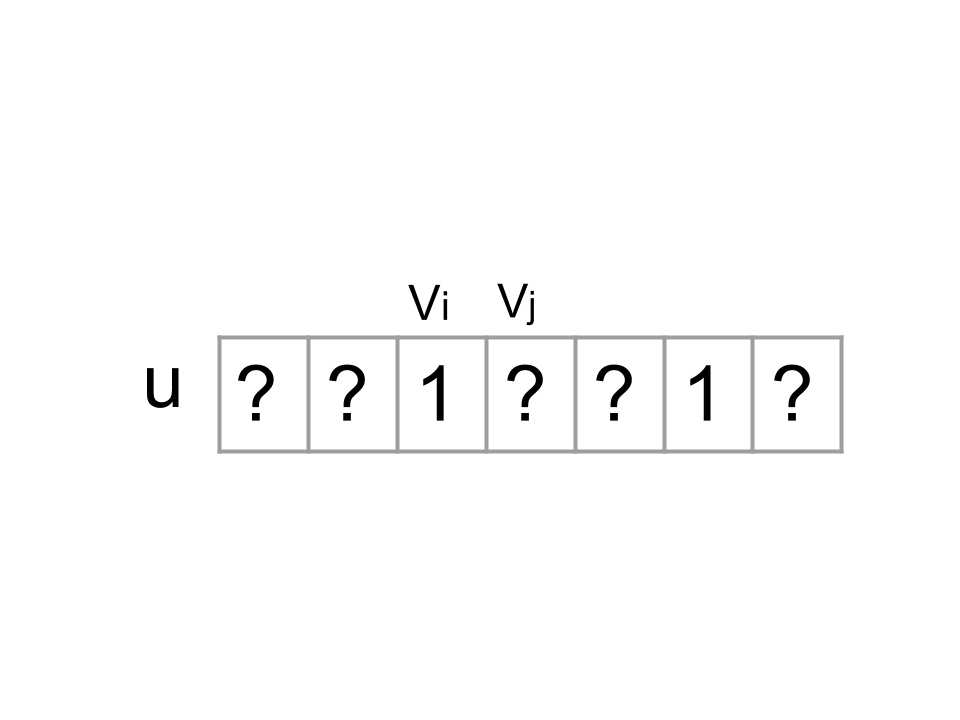
\includegraphics[width=3in]{pairwise}
			\end{figure}
			\vspace{-6em}
			\hspace{4em} \textcolor{red}{user $u$ prefers item $v_i$ over  $v_j$}
			
		\column{.5\textwidth}
		\begin{itemize}
			\item define the pairwise preference of user $u$ as:
			\begin{equation}
			p \left( i \succ_u j \right) := f \left( x_{uij} \right),
			\end{equation}
			where $f \left(x\right) = 1/\left(1+exp\left(-x\right)\right)$, $x_{uij} := \hat{r}_{uij} = \hat{r}_{ui} -\hat{r}_{uj}$.
		\end{itemize}
		
	\end{columns}
\end{frame}

\subsection*{Prediction Rule}
\begin{frame}{Prediction Rule}
	\begin{itemize}
		\vspace{2em}
		\item The predicted rating $\hat{r}_{ui}$ of user $u$ on item $i$ :
		\begin{equation}
		\hat{r}_{ui} = U_{u\cdot}V_{i\cdot}^T + b_i
		\end{equation}
		\begin{centering}
			\begin{figure}
				\vspace{-7em}
				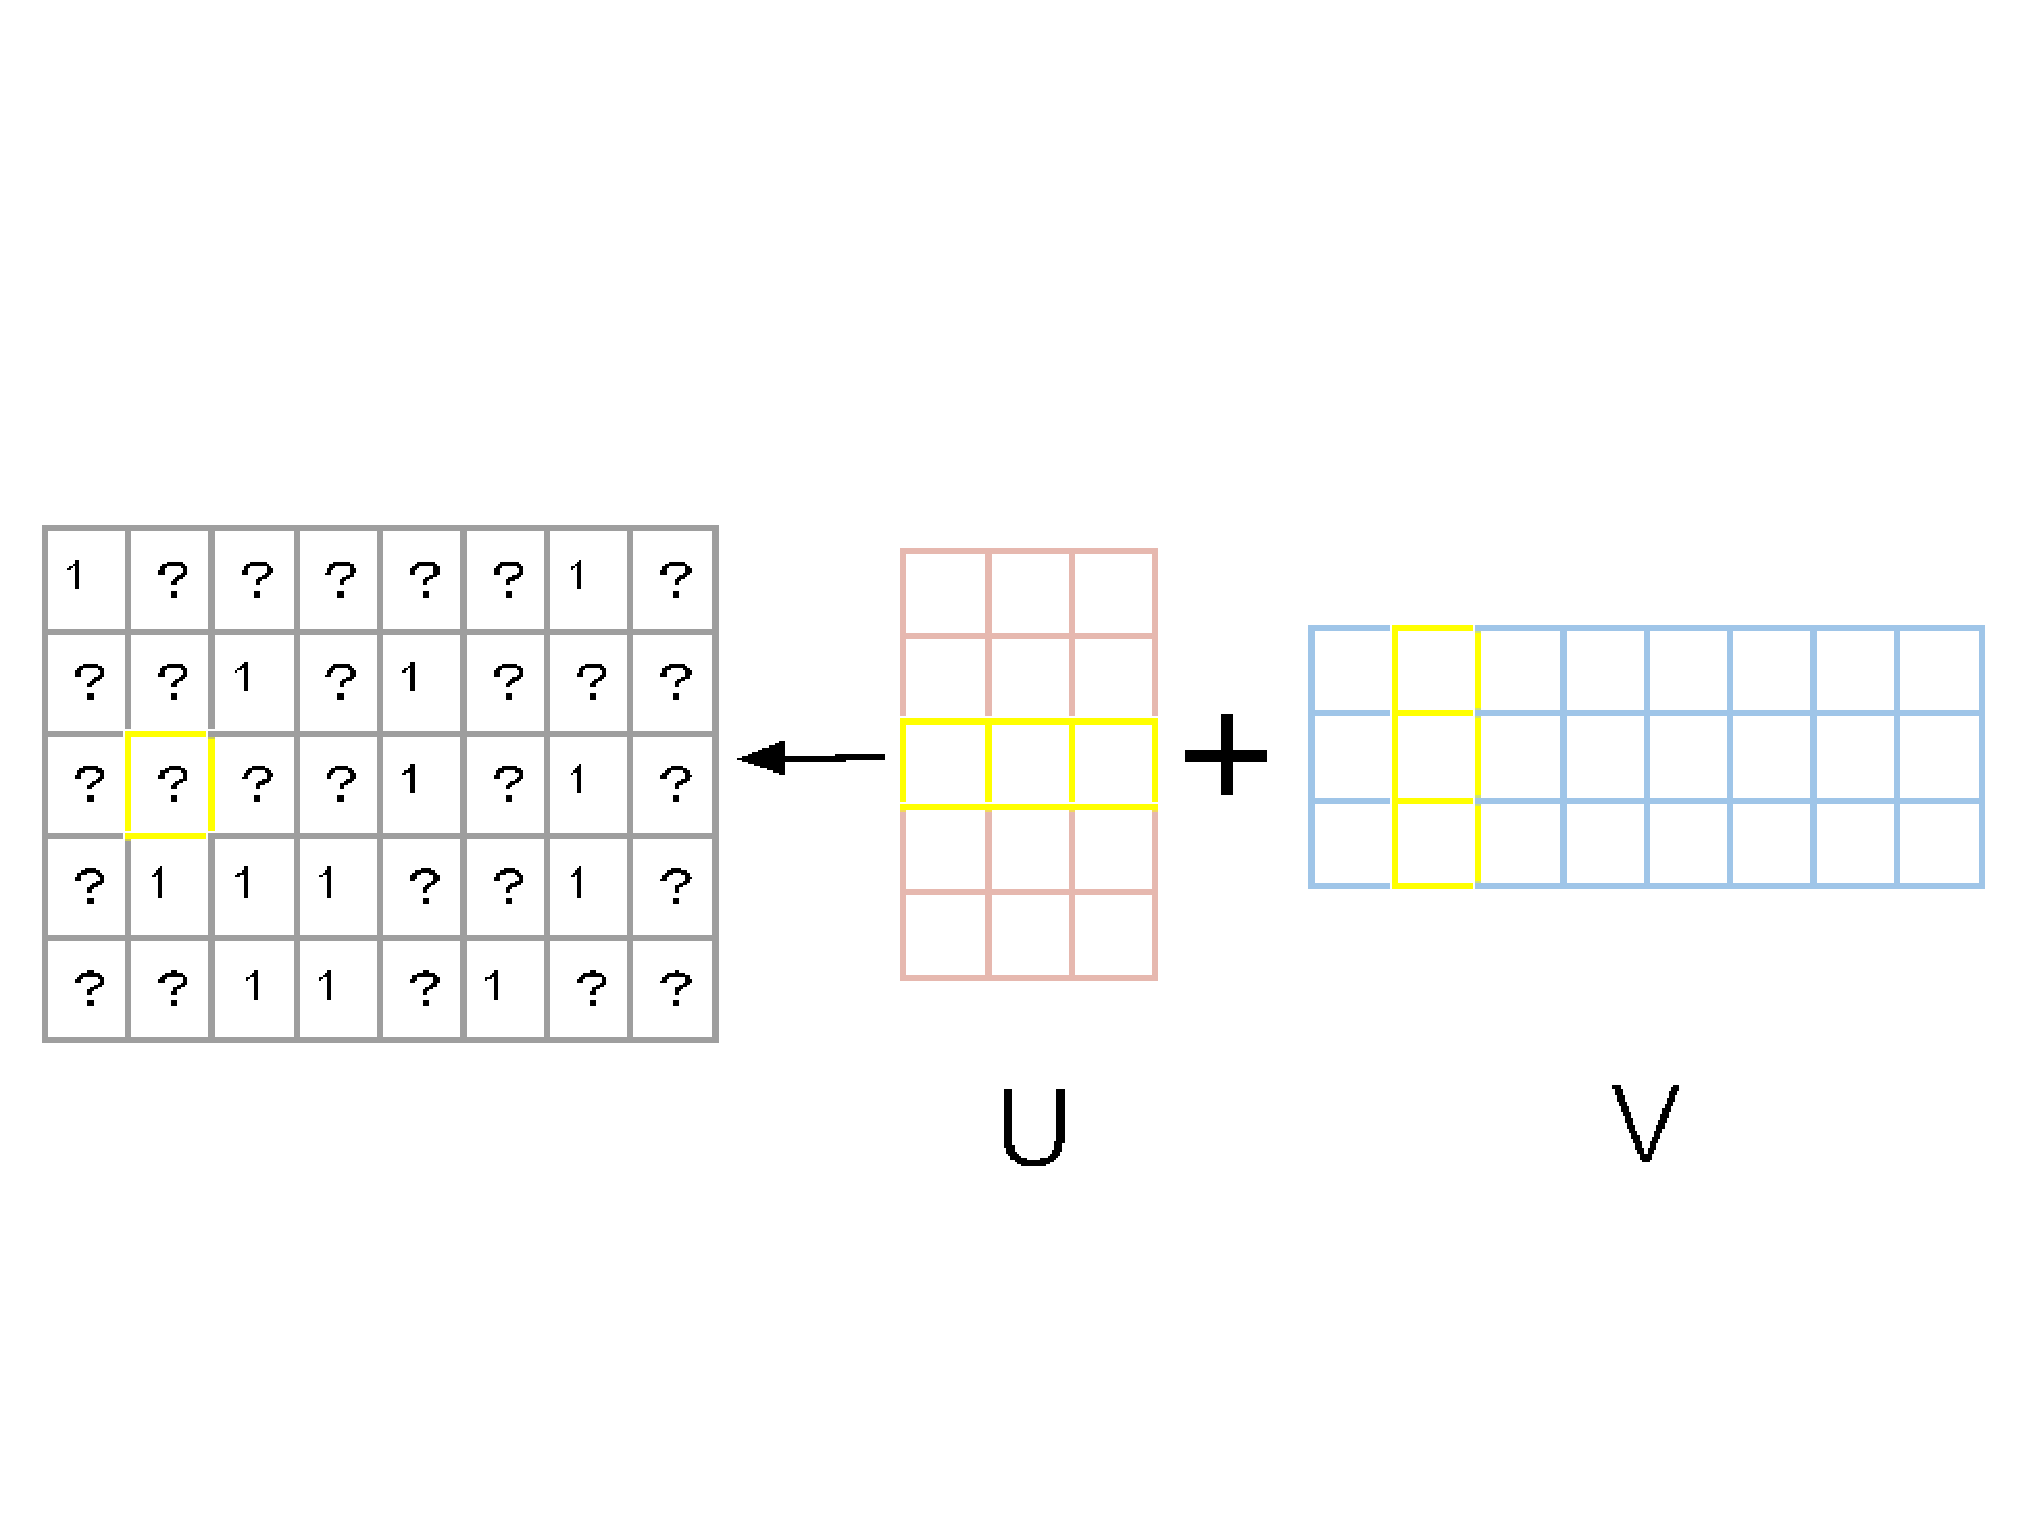
\includegraphics[width=4in]{uv}
			\end{figure}
		\end{centering}
	\end{itemize}
	
\end{frame}


\subsection*{Likelihood of Pairwise Preference}
\begin{frame}{Likelihood of Pairwise Preference}
	\begin{itemize}
		
		\setlength{\itemsep}{2ex plus0.2ex}
		
		\item The random variable $x$ with Bernoulli distribution :
		
		\scalebox{0.8}{
			\parbox{1.2\textwidth}{
				\begin{equation}
				Ber\left(x|p \right)=p^x\left(1-p \right)^{1-x} \qquad  \text{for}\  x \in \{0,1\},p \in [0,1]
				\end{equation}
			}
		}
		
		
		\item The Bernoulli distribution of binary random variable $x \left(\left(u,i\right) \succ \left(u,j\right)\right)$ is
		defined as follows :
		%%%%公式太长了先放入到一个盒子中parbox,在对盒子进行缩放scalebox
		\scalebox{0.8}{
			\parbox{1.2\textwidth}{
					\begin{equation}
					\label{eq4}
					\begin{aligned}
					LPP_u  
					&= \prod_{ \ i,j \  \in \  \mathcal{I}}p\left(\hat{r}_{ui} > \hat{r}_{uj}\right)^{x \left(\left(u,i\right) \succ \left(u,j\right)\right)} \left[1-p\left(\hat{r}_{ui} > \hat{r}_{uj}\right)\right]^{1-x \left(\left(u,i\right) \succ \left(u,j\right)\right)}\\
					&= \prod_{\left(u,i\right) \succ \left(u,j\right)}p\left(\hat{r}_{ui} > \hat{r}_{uj}\right)\prod_{\left(u,i\right) \preceq \left(u,j\right)}\left[1-p\left(\hat{r}_{ui} > \hat{r}_{uj}\right)\right]
					\end{aligned}
					\end{equation}
				}
		}
		where \textcolor{red}{$(u,i) \succ (u,j)$ means that user $u$ prefers item $i$ to item $j$}.
	\end{itemize}
\end{frame}




\subsection*{Objective Function}
\begin{frame}{Ojective Function}
	\begin{itemize}
		\item  Given a set of pairwise preference $D_S$ , the
		goal of BPR is to maximize the likelihood of all pairwise
		preference:
		\begin{equation}
		arg \ \max_{\substack \Theta } \prod_{\left(u,i,j\right) \in D_S} p\left(i \succ_u j\right),
		\end{equation}
		which is equivalent to minimize the negative log likelihood:
		\begin{equation}
		\label{eqbprojc}
		L_{feedback} = - \sum_{\left(u,i,j\right) \in D_S}\ln f \left( \hat{r}_{uij}\right) + \lambda\|\Theta\|^2,
		\end{equation}
		where $\hat{r}_{uij} = \hat{r}_{ui} - \hat{r}_{uj}$, $\Theta$ denotes the set of all latent vectors and $\lambda$ is a hyper-parameter.
	\end{itemize}
\end{frame}

\begin{frame}{Ojective Function}
	\begin{itemize}
		\item Specifically, Eq\eqref{eqbprojc} is to minimize the following objective function  : 
		\begin{equation}
		\min_{\substack\Theta}\sum_{u\in\mathcal{U}}\ \sum_{i\in\mathcal{I}_u}\sum_{j\in\mathcal{I}\setminus\mathcal{I}_u}\Phi_{uij}
		\end{equation}
		where
		$\Phi_{uij}
		= 
		- \ln f \left(\hat{r}_{uij}\right) 
		+ \frac{\alpha_u}{2}\|U_{u\cdot}\|^2
		+ \frac{\alpha_v}{2}\|V_{i\cdot}\|^2
		+ \frac{\alpha_v}{2}\|V_{j\cdot}\|^2
		+ \frac{\beta_v}{2}\|b_{i}\|^2
		+ \frac{\beta_v}{2}\|b_{j}\|^2$, $\Theta = \{U_{u\cdot},V_{i\cdot},b_i\}
		$ denotes the parameters to learn.
	\end{itemize}
\end{frame}



\subsection*{SGD}
\begin{frame}{SGD}
	\begin{itemize}
		
		\setlength{\itemindent}{-2ex}
		
		\item For a randomly sampled triple $\left(u,i,j\right)$, calculate the partial derivative for $U_{u\cdot}$:
		
		\vspace{3ex}
		
		\scalebox{0.8}{
			\parbox{1.2\textwidth}{
				\begin{equation}
				\hspace{-9ex}
				\begin{aligned}
				\bigtriangledown U_{u\cdot} 
				= \frac{\partial \Phi_{uij}}{\partial U_{u\cdot}}
				&=-\frac{\partial \ln f\left(\hat{r}_{uij}\right)}{\partial f\left(\hat{r}_{uij}\right)} 
				\frac{\partial f\left(\hat{r}_{uij}\right) }{\partial \hat{r}_{uij}} 
				\frac{\partial \hat{r}_{uij}}{\partial U_{u\cdot}}
				\ + \  \alpha_uU_{u\cdot}\\
				&= -\frac{1}{f\left(\hat{r}_{uij}\right)} 
				\frac{\partial f\left(\hat{r}_{uij}\right) }{\partial \hat{r}_{uij}} 
				\frac{\partial \hat{r}_{uij}}{\partial U_{u\cdot}}
				\ + \  \alpha_uU_{u\cdot}\\
				&= -\frac{1}{f\left(\hat{r}_{uij}\right)} 
				{f\left(\hat{r}_{uij}\right) f\left(-\hat{r}_{uij}\right)}
				\frac{\partial f\left(\hat{r}_{ui} - \hat{r}_{uj}\right) }{\partial U_{u\cdot}} 
				\ + \ \alpha_uU_{u\cdot}\\
				&= -{f\left(-\hat{r}_{uij}\right)} \frac{\partial f\left[\left(U_{u\cdot}V_{i\cdot}^T+b_i\right) - \left(U_{u\cdot}V_{j\cdot}^T+b_j\right)\right] }{\partial U_{u\cdot}} 
				\ + \ \alpha_uU_{u\cdot}\\
				&= -{f\left(-\hat{r}_{uij}\right)} \left(V_{i\cdot} - V_{j\cdot}\right)  
				\ + \  \alpha_uU_{u\cdot}\\
				\end{aligned}
				\end{equation}
			}
		}
	\end{itemize}
\end{frame}
\begin{frame}{SGD}
	\begin{itemize}
		\item For the rest of parameters, we have the partial derivatives:
		\begin{align} %align环境不要有空行
		\bigtriangledown V_{i\cdot} &= \frac{\partial \Phi_{uij}}{\partial V_{i\cdot}}=-f\left(-\hat{r}_{uij}\right)U_{u\cdot} + \alpha_vV_{i\cdot}\\
		\bigtriangledown V_{j\cdot} &= \frac{\partial \Phi_{uij}}{\partial V_{j\cdot}}=-f\left(-\hat{r}_{uij}\right)\left(-U_{u\cdot}\right) + \alpha_vV_{j\cdot}\\
		\bigtriangledown b_i        &= \frac{\partial \Phi_{uij}}{\partial b_i} =-f\left(-\hat{r}_{uij}\right)+\beta_vb_i\\
		\bigtriangledown b_j        &= \frac{\partial \Phi_{uij}}{\partial b_j} =-f\left(-\hat{r}_{uij}\right)\left(-1\right)+\beta_vb_j
		\end{align}
		where $ \hat{r}_{uij} = \hat{r}_{ui} - \hat{r}_{uj}$. 
	\end{itemize}
\end{frame}
\begin{frame}{Update Rules}
	\begin{itemize}
		\item For a randomly sampled triple $(u,i,j)$, we have the update rules,
		\begin{align}
		\label{eq10}
		U_{u\cdot} &= U_{u\cdot} - \gamma\bigtriangledown U_{u\cdot}\\
		V_{i\cdot} &= V_{i\cdot} - \gamma\bigtriangledown V_{i\cdot}\\
		V_{j\cdot} &= V_{i\cdot} - \gamma\bigtriangledown V_{j\cdot}\\
		b_{i\cdot} &= b_i - \gamma\bigtriangledown b_{i}\\
		b_{j\cdot} &= b_j - \gamma\bigtriangledown b_{j}
		\end{align}
		where $\gamma$ is the learning rate.
	\end{itemize}
\end{frame}

\subsection*{SGD for BPR}
\begin{frame}{The SGD algorithm for BPR}
	\IncMargin{1em}%将行号对齐到里面
	\begin{algorithm}[H]%beamer中使用算法,需要[H]选项否则会出现outer mode错误
		\SetAlgoNoLine %不要算法中的竖线
		\BlankLine
		
		initialize the model parameter $\Theta$\;
		\For {$t_1 = 1,\cdots,T$}{
			\For {$t_2 = 1,\cdots, |\mathcal{P}|$}{
				Randomly pick up a pair $\left(u,v_i\right) \in \mathcal{P}$\;
				{\color{red}{Randomly pick up an item $v_j$ from $\mathcal{I} \setminus \mathcal{I}_{u}^+$}\;}
				Calculate the gradients via Eq.(8-12)\;
				Update the model parameters via Eq.(13-17)\;
			}	
		}
		\caption{The SGD algorithm for BPR}
		\label{al1}%label 放置的位置有讲究, 放后面
	\end{algorithm}
	\DecMargin{1em}
	
\end{frame}


	\section{推荐系统概述}

\subsection{主要符号表}

\begin{table}[htbp]%[htbp]表格参数设置,固定位置
	\setlength\tabcolsep{2pt}
	\renewcommand\arraystretch{1.3}%改变行高
	\caption{主要符号表}
	\label{tab1}
	\begin{center}
		
		\begin{tabular}{cc}
			
			\Xhline{1.2pt}
			常用符号                    & 意义\\
			\hline
			$s$                         & user number \\
			$t$                         & item number \\
			$u$                         & user \\
			$v$                         & item \\
			$u_m$                       & the specified user $m$\\
			$v_i$                       & the specified item $i$\\
			$v_j$                       & the specified item $j$ \\
			$b_i$                       & item bias \\
			${r}_{ui}$                  & real rating of user $u$ on item $i$\\
			$\hat{r}_{ui}$              & predicted rating of user $u$ on item $i$\\
			$\hat{r}_{uj}$              & predicted rating of user $u$ on item $j$\\
			$e_i$                       & entity, e.g., user $u$ or item $v$\\ 
			$T$                         & iteration number in the algorithm\\
			$k \in \mathbb{R}$          & number of lentent dimensions \\
			$r\left(j\right)$           & the ranking place of the item $v_j$\\
			$\mathcal{P}$               & (user, item) pairs in training data \\
			$\mathcal{P}^{te}$          & (user item) pairs in test data\\ 
			$\mathcal{U}$               & the whole user set\\
			$\mathcal{I}$               & the whole item set \\
			$\mathcal{I}_u^{re}$        & recommended items for user $u$\\
			$\mathcal{I}_u^{te}$        & selected items by user $u$ in test data\\
			$\mathcal{I}_u^{tr}$        & selected items by user $u$ in training data\\
			$\mathcal{I}_{u_m}^+$       & the set of items selected by the user $u_m$ \\
			$U \in \mathbb{R}^{s \times k } $             & user-specific lantent matrix \\
			$V \in \mathbb{R}^{t \times k } $             & item-specific lantent matrix \\
			$U_{u \cdot } \in \mathbb{R}^{1 \times k } $  & 
			user-specific latent feature vector \\
			$V_{v \cdot } \in \mathbb{R}^{1\times k}$     &
			item-specific lantent feature vector\\
			$Y^e = \left[y_1^e,y_2^e,y_3^e,\cdots\right]$ & latent representation of entities \\
			$y_i^e \in \mathbb{R}^{1\times k}$            & 
			the latent vector of entity $e_i$ \\
		    $\mathcal{C} = \{c_1,c_2,\cdots,c_k\}$        & categories\\
			$D_S := \{\left(m.i,j\right) | v_i \in \mathcal{I}_{u_m}^+ \wedge v_j \in \mathcal{I} \setminus \mathcal{I}_{u_m}^+\}$                        &  
			the set of all pairwise preference\\
			\Xhline{1.2pt}
			
		\end{tabular}
	\end{center}
\end{table}
表\ref{tab1}中列举了大部分在本文中使用的符号及其意义。




\subsection{推荐系统纵览}

自从20世纪90年代中期第一篇关于协同过滤(Collaborative Filtering)的研究文章\cite{DBLP:conf/cscw/ResnickISBR94}出现以后,推荐系统就开始成为了一个重要且有趣的研究主题。协同过滤通过收集推荐系统中相似用户的偏好进行推荐,而生成近邻用户(neighbourhood formation)是协同过滤中非常重要的一个方面\cite{DBLP:journals/isci/KardanE13,DBLP:conf/icic/LeePP07}.近邻用户生成的目的是为每个用户找到一些相似的用户群或其最近邻,然后基于有着相似偏好的近邻用户推荐产品或服务\cite{DBLP:journals/eswa/ZhengL11,DBLP:journals/ecra/ChoiYKS12}。这里的近邻(neighbourhood)是指那些对于我们将要为之提供推荐建议的用户所感兴趣的物品有过相似交互行为的其他用户。在这里,我们把需要为之提供推荐的用户成为目标用户,那么通过比较目标用户与其近邻评分,就可以做出最终的推荐\cite{DBLP:journals/eswa/AcilarA09,kim2011recommender}。当缺乏用户评分数据的时候,协同过滤就会遇到所谓的稀疏性问题,这将导致推荐效果变得很差。因此,在推荐系统中预防稀疏性问题非常重要。为此一个很重要的途径便是从隐式反馈(比如用户的购买行为,上线时间,历史浏览记录)数据中提取用户的偏好信息来降低协同过滤对于用户评分数据的依赖,同时提高推荐效果\cite{DBLP:conf/icdm/HuKV08,DBLP:journals/eswa/AlbadviS09}。隐式反馈数据能够通过对于用户行为的观测提供更多的信息来降低评分数据不充分的影响\cite{rafeh2012adaptive,DBLP:journals/eswa/ZhengL11}。另一方面,协同过滤推荐技术的用户画像(user profile)通过用户对于物品的评分得以构建。为了降低协同过滤对于评分数据的依赖,用户行为(user activity)也已经成为研究调查的一个重要关注点,也就是说通过挖掘用户偏好的经验性知识来构建更加精确的用户画像(user profile)\cite{lee2010collaborative,DBLP:journals/eswa/ZhengL11,kim2011recommender,DBLP:journals/ecra/ChoiYKS12}。




\subsection{典型推荐算法概述}

推荐系统通过识别用户的需求与偏好为其推荐合适的产品或服务。目前国内外关于推荐系统的研究下已衍生了很多推荐算法,这些推荐算法通常可以分为三类:基于内容的推荐(Content-based recommendations), 协同过滤(Collaboratibe Filtering)和混合型(Hybrid approches)推荐.
 
 
\subsubsection{基于内容的推荐系统}

基于内容信息的方法\cite{gantner2010learning,rendle2012factorization,hong2013co}来学习个体的隐式表达(latent representation)并缓解冷启动(cold start)问题。比如,在FM\cite{rendle2012factorization}中各种属性信息被放到特征矩阵中,然后通过对于评分数据回归分析相关属性。

基于内容的推荐系统从用户与物品的content profile之间的相似度出发进行推荐。他们从研究推荐系统中个体的内容信息角度进行分析。通常这类方法利用个体的内容信息,比如物品属性,用户文本,或照片的像素点,主要利用探索启发式(heuristics)的方法。在\cite{balabanovic1997fab,lang1995newsweeder,mooney2000content}中,他们使用诸如cosine similarity的方式来衡量相似度,然后推荐在内容上与用户过去所喜欢的相类似的物品。在\cite{pazzani1997learning}中,基于物品内容信息并由用户标注的标签:“相关(relevant)”或者是“不相关(irrelevant)”,作者学习了一个贝叶斯分类器来对没有标注的物品进行分类。 近来,也有很多社交媒体(social media)相关的推荐系统关注content-based推荐方法并对其进行了很多研究。比如,在\cite{li2009learning,liu2009tag}中通过基于可视性的内容相似度考虑它的最近邻标签, 然后来为目标图像推荐标签。\cite{mei2007videoreach}提出了一个在线视频的推荐系统,而该系统则利用了在用户与视频间点击数据的多模态的内容关联度。

但是,这些基于内容的推荐方法大都具有以下局限性: 第一, 它们必须有足够的信息构建一个分类器, 并且显然会被推荐物品的特征所局限; 第二, 它们推荐的物品, 在内容上往往与用户已经有过评分行为的物品很相似, 显然这就会导致了较低的推荐多样性。


\subsubsection{基于协同过滤的推荐系统}
协同过滤(Collaborative Filtering)方法通过挖掘用户的评分历史来预测用户的偏好。它们并不需要内容信息(content information),并且能够发现一些基于内容的推荐方法所不能发现的一些有趣的联系。通常来说,协同过滤基于这样一个基本的设想:相似的用户对于相似的物品有着相似的行为\cite{adomavicius2005toward,su2009survey}。这里的“相似”并不同于content-based方法中的内容相似度(content similarity), 它指的是相似的评分偏好(similar rating preference)。

协同过滤方法可大致分为两类:memory-based methods, model-based methods。memory-based方法\cite{breese1998empirical,herlocker1999algorithmic,linden2003amazon,sarwar2001item}通常通过搜寻相似的用户或商品去进行推荐。而其相似度则是经由评分历史计算而得。memory-based方法也可进一步的被分为user-based和item-based两类方法。通过与当前用户有着相似偏好的其他用户进行推荐即为user-based, 通过推荐与当前用户喜欢过的物品所相似的物品即为item-based。不过,当缺乏用户评分数据的时候,协同过滤就会遇到叫做稀疏性的一个问题,这将很容易导致推荐效果变得很差。因此,在推荐系统常常需要应对稀疏性这一大难题。应对稀疏性问题一个重要的途径便是从隐式反馈(implicit feedback)(比如用户的购买行为,上线时间,历史浏览记录)数据中提取用户的偏好信息来降低协同过滤对于用户评分数据的依赖,当然这往往同时也能够提高推荐效果\cite{DBLP:conf/icdm/HuKV08,DBLP:journals/eswa/AlbadviS09}。另外, 相对于显式反馈,隐式反馈的数据更易采得也更丰富。隐式反馈能够通过对于用户行为的观测提供更多的信息来降低评分数据不充分的影响\cite{rafeh2012adaptive,DBLP:journals/eswa/ZhengL11}。这时其实也就是变成我们所谓的单类协同过滤(One-class Collaborative Filtering)问题。

OCCF问题的最典型特征是仅能够观测到正向采样(positive examples), 比如用户的点击行为, 浏览行为,同时数据分类往往非常不均衡, 比如用户点击过物品可能只是占到整个物品集合的很小一部分。我们把用户未有过交互行为的物品,比如未点击过的物品,叫做negative examples. 那么如何从大量未有过交互行为的物品集合中针对negative examples进行采样与建模是很多问题的关键所在。在前人的一些工作中,有几种直观的策略来处理这个问题。其实一个最常见的做法是将所有缺失的数据视作negative examples,显然这将导致推荐结果具有偏差,因为很多缺失数据很多可能是positive examples。另一种做法是所缺失的数据是做未知的,这将导致协同过滤模型仅利用了positive examples。近来的一些研究中,一些关于OCCF的研究人员将重点放到了对于negative examples的建模上[19,34,35,44]。他们的一个基本的想法是将所缺失的数据视作是negative,但是给出了将其视作negative的一个概率权重。不过,他们当中的部分做法仅仅是通过简单地观测历史反馈的概率属性来区分negative examples。比如,[19,34],他们计算了每个用户给多少物品评过分,每个物品被多少用户评过分,由此来计算一个权重。进一步的说,他们认为如果一个用户浏览过的物品越多,那么他没有浏览过的物品便更大可能是negative类型;如果一个物品被越少的用户浏览过,那么这个物品相关缺失数据便更小可能是negative, 这种做法仍然是略显粗糙。

协作型方法\cite{rendle2009bpr,yu2013recommendation,zhong2014adaptive}通过处理大量的用户与物品间的交互信息,比如隐式反馈和显式的评分(也叫作协同信息)。这些方法不同于memory-based方法,model-based方法采用机器学习与概率统计的技术从已有的用户评分去学习一个模型,再将模型应用到推荐中。其中包括有隐语义模型(latent semantic models), 图模型(graphical models),贝叶斯模型(Bayesian models), 聚类模型(clustering models).在众多的model-based方法中,低秩矩阵分解(low-rank Matrix Factorization)由于在可扩展性与精确度方面的优势已经获得了许多研究者的关注。其实分解的方法在个性化的推荐系统中很常见。他们可以被用来处理推荐系统中收集的各种信息,比如隐式反馈\cite{hu2008collaborative,rendle2009bpr},物品属性\cite{gantner2010learning,rendle2012factorization},用户画像\cite{hong2013co}和社交信息\cite{ma2011recommender}。其中矩阵分解基于用户的偏好可以被一小部分因子表示,通过从user-item rating matrix来学习user与item一个低秩隐含因子,然后利用它们去预测未被观测到的ratings。

矩阵分解\cite{girase2015role}及其一些扩展方法\cite{li2010improving,gemulla2011large,zhang2014temporal}是用来处理协同信息的非常典型的分解方法, 它通过分解协同信息并试图在一个共享的隐式空间学习用户与物品的隐式表达。比如,隐式矩阵分解\cite{hu2008collaborative}通过为每个user-item pair计算一个适应性的信任权重来扩展基础的BPR处理隐式反馈。尽管通过扩展BPR能够应对隐式反馈问题,但是由于在隐式反馈数据集中普遍存在的数据倾斜(data skew)问题(正反馈数量常常不到总数的1\%), 他们很容易陷入过拟合问题。为了缓解数据倾斜与推荐系统的隐式反馈学习,Bayesian Personalized Ranking (BPR)\cite{rendle2009bpr}和它的一些扩展方法\cite{pan2013gbpr,qiu2014item,rendle2014improving}被提出,其所基于的假设为:相比于未选择的物品用户更感兴趣已经选择的物品。这样假设会产生大量的训练数据,因此对应的学习算法通常基于均匀采样用户物品对的随机梯度下降。但是不同的训练采样可能会对参数学习产生不同的影响,均匀采样策略往往会产生大量低效的训练采样并导致收敛变得缓慢。尤其是当物品数量很大和物品的流行度有着长尾分布(long distribution)\cite{feldmann1997fitting}的时候,均匀采样策略将会导致极其缓慢的收敛。因此,BPR的作者Rendle进一步研究了长尾效应并利用它提出了非均匀的物品采样器\cite{rendle2014improving}。对于给定的一个用户,他们计划挑选出那些在某一领域很流行并且尚未被该用户选择过的物品来构成训练对。理论上,这种采样方式很耗时,因为它将物品的隐式因子当做物品流行度的指示器并且需要在每轮迭代的每个区域对物品进行重新排序。为了考虑运行效率,Rendle不得不减少重新排序的时间来妥协推荐性能。另一方面,为了获得一个通用的加速BPR学习的方案,\cite{zhong2014adaptive} 尝试根据一个在两个不同未选择过的物品上的偏好差别来选取那些富含信息的训练对。但是,由于真实世界的数据集里物品数往往极其庞大,这种策略不得不在计算偏好差别上花费大量的时间。因此,\cite{rendle2014improving,zhong2014adaptive}都陷入了平衡算法效率与性能表现的两难境地。在本课题中所研究的采样策略在效率与性能两方面都表现了很好的效果,并且有潜力加速BPR的学习。

传统的协同过滤对于评分预测问题往往能够取得很好的效果,比如Netflix的电影推荐。但是,它受制于一个众所周知的问题: 冷启动,当一个新的物品或用户进入系统时由于几乎无法获得任何评分记录, 在此种情况下推荐效果往往很不理想。为了缓解推荐系统中的冷启动问题,Map-BPR\cite{gantner2010learning}扩展了BPR框架,他们学习了一个将内容信息空间映射到隐式空间的一个映射关系。然后,Map——BPR利用学习到了这个映射学习那些缺乏协同信息的新个体的隐式因子。不过,Map-BPR将隐式因子的学习分割为两个不相关的部分。这会导致在隐式反馈数据集中的个体的隐式因子仅仅指示协同属性而不会显示内容属性。为了获得更可信的隐式因子,在本课题的研究方法在同一个学习过程中研究了通过协同信息与内容信息学习个体的隐式因子。

\subsubsection{混合式推荐系统}
混合方法尝试将基于内容与协同过滤的推荐方法结合起来应对它们的局限性。\cite{burke2007hybrid}通过将基于内容与协同过滤的预测结果进行线性组合设计了一个混合推荐模型。\cite{schein2002methods}提出从概率混合的角度将协同过滤与基于内容的推荐方法进行统一。近来也有很多工作都重点关注了社交媒体推荐(social media recommendation),而他们中的大部分都采用了混合方法,在挖掘社交媒体内容的同时考虑了用户的历史行为来获得更高的推荐准确度。\cite{wang2013joint}为在线社交网络中的视频推荐(video recommendation)设计了一个组合式的社交内容推荐框架. 他们的方法通过利用社交网络信息(social network information)与内容信息(content information), 提出一个user-conetnt matrix填充冷启动中的user-video条目。\cite{tiemann2007towards}研究利用了集成学习(ensemble learning)方法,在音乐推荐中将基于物品协同过滤结果与基于内容方法的结果进行融合。




\subsection{推荐系统评价指标}
所谓评价指标主要包括“技术评价指标”和“业务评价指标”。技术评价指标包括诸如 RMSE\footnote{RMSE: \textbf{R}oot \textbf{M}ean \textbf{S}quared \textbf{E}rror, 均方根误差}、MAE\footnote{MAE: \textbf{M}ean \textbf{A}bsolute \textbf{E}rror, 平均绝对误差}、
NDCG\footnote{NDCG: \textbf{N}ormalized \textbf{D}iscounted \textbf{C}umulative \textbf{G}ain}、MAP\footnote{MAP: \textbf{M}ean \textbf{A}verage  \textbf{P}recision, 平均准确率 }、Recall、Precision 等,业务评价指标如成交转化率、用户点击率等。\cite{xiangliang}也介绍了推荐系统中的很多评测指标。这些评测指标可用于评价推荐系统各方面的性能。,它们包括用户满意度、预测准确度、覆盖率、多样性、实时性、健壮性等等。其中有些可以通过计算来定量衡量,有些则只能定性描述,有些可以通过离线实验计算,有些需要通过用户
调查获得,还有些只能在线评测。这里主要介绍在技术评价指标中, 评分预测与TopN推荐的预测准确度定义。




\subsubsection{评分预测}
\begin{figure}[htbp]
	% caption放上面就会显示在图的上方,出现在下面就是出现在图的下方
	\label{gra1}
	\begin{center}
		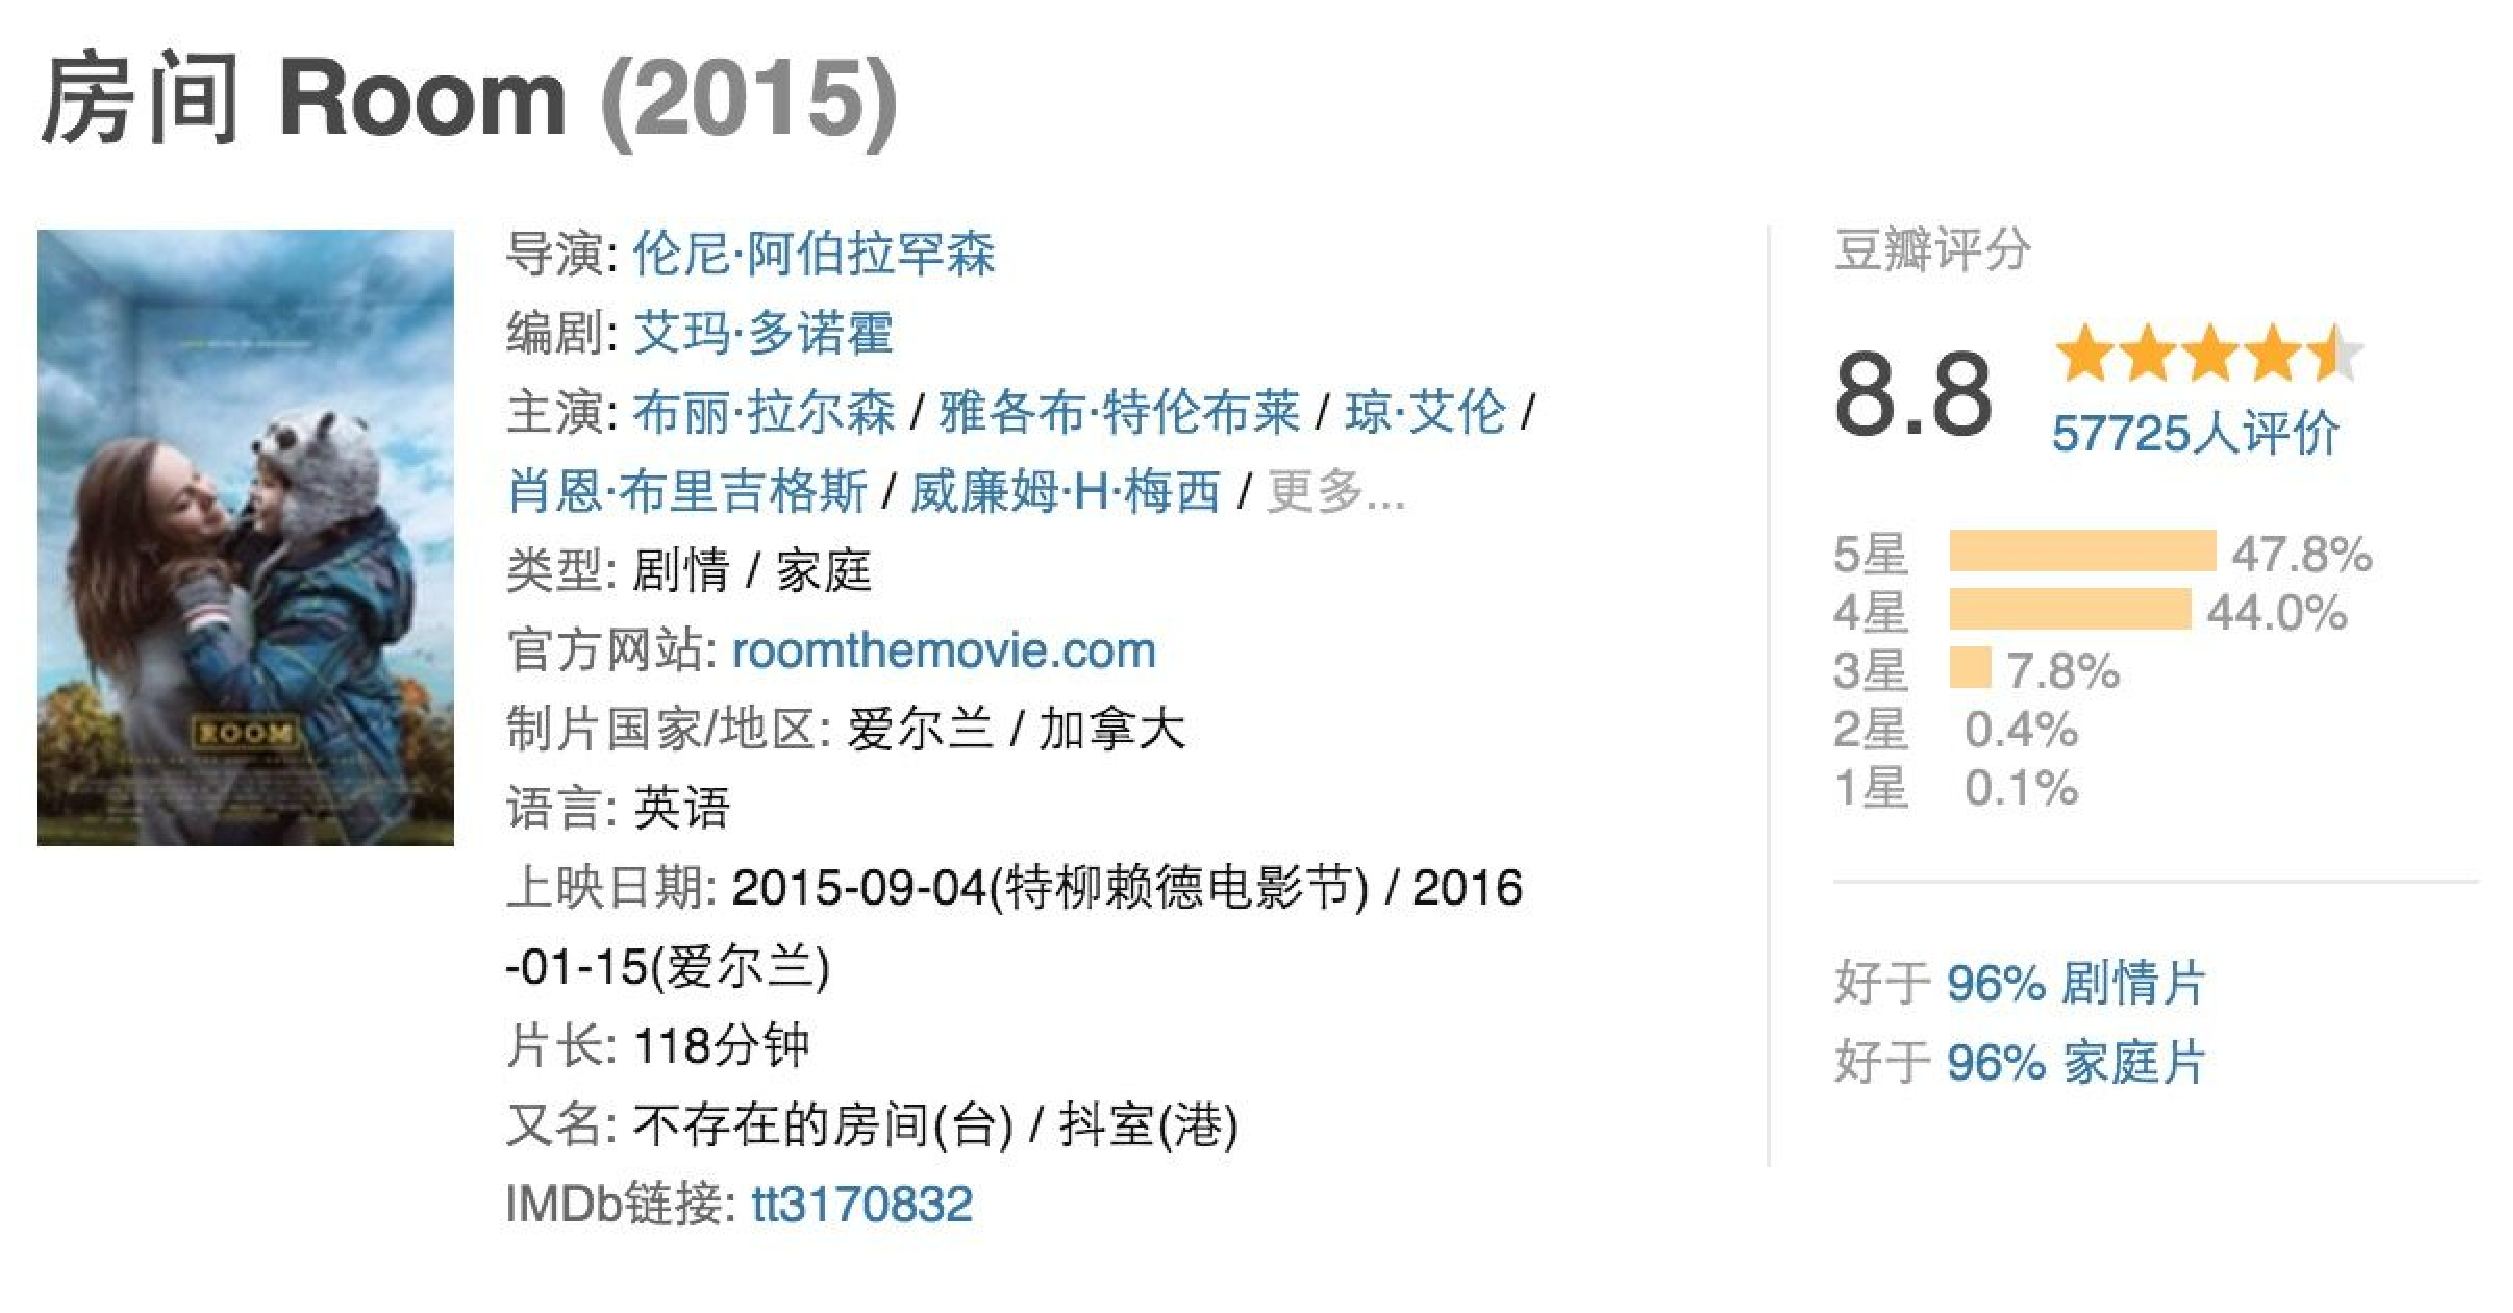
\includegraphics[width=4in]{rating}
		\caption{用户评分}
	\end{center}
\end{figure}
很多提供推荐服务的网站都有一个让用户给物品打分的功能。那么,如果
知道了用户对物品的历史评分,就可以从中习得用户的兴趣模型,并预测该用户在将来看到一个
他没有评过分的物品时,会给这个物品评多少分。预测用户对物品评分的行为称为评分预测。

评分预测的预测准确度一般通过RMSE和MAE计算。对于
测试集中的一个用户$u$和物品$i$,令$r_{ui}$是用户$u$对物品$i$的实际评分,而$\hat{r}_{ui}$是推荐算法给出的预测评
分,那么 RMSE 的定义为:
\begin{equation*}
RMSE = \frac
{\sqrt{{\sum_{\left(u,i\right) \in \mathcal{P}^{te}} \left(r_{ui} - \hat{r}_{ui}\right)^2}}} {|\mathcal{P}^{te}|}
\end{equation*}
MAE 采用绝对值计算预测误差,它的定义为:
\begin{equation*}
MAE = \frac{{\sum_{\left(u,i\right) \in \mathcal{P}^{te}}} |r_{ui} - \hat{r}_{ui}|}
	{|\mathcal{P}^{te}|}
\end{equation*}

关于 RMSE 和 MAE 这两个指标的优缺点, Netflix 认为 RMSE 加大了对预测不准的用户物品评
分的惩罚(平方项的惩罚),因而对系统的评测更加苛刻。研究表明,如果评分系统是基于整数
建立的(即用户给的评分都是整数),那么对预测结果取整会降低 MAE 的误差
。


\subsubsection{TopN推荐}
\begin{figure}[htbp]
	
	\label{gra2}
	\begin{center}
		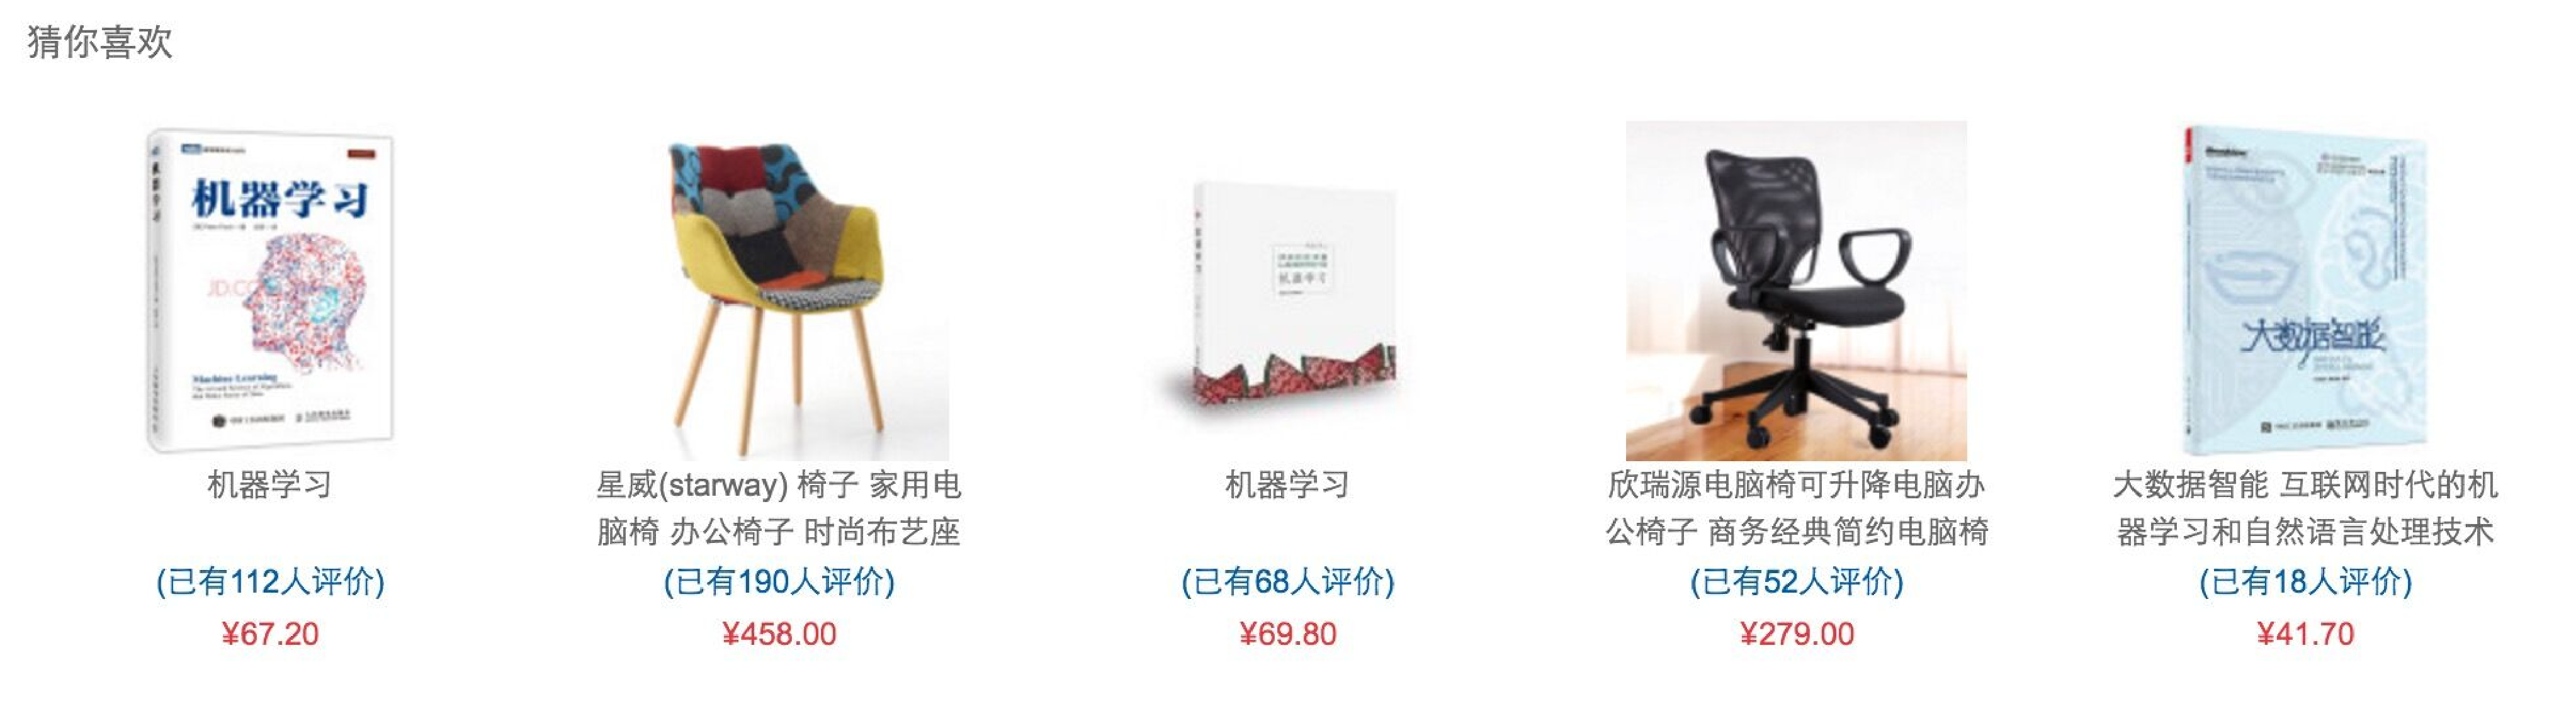
\includegraphics[width=6in]{topn}
		\caption{TopN推荐}
	\end{center}
\end{figure}
网站在提供推荐服务时,一般是给用户一个个性化的推荐列表,例如购物网站上的热门推荐,这种推荐叫做 TopN 推荐。在现实场景下,TopN推荐也是更常见的一种推荐形式。

TopN 推荐的预测准确率一般通过准确率(precision)/召回率(recall)衡量。
对于用户$u$, 推荐列表$\mathcal{I}_u^{re}$的准确率定义为:
\begin{equation*}
Precision_u = \frac{|\mathcal{I}_u^{re} \cap \mathcal{I}_u^{te}|}{|\mathcal{I}_u^{re}|}
\end{equation*}
其召回率定义为:
\begin{equation*}
Recall_u = \frac{|\mathcal{I}_u^{re} \cap \mathcal{I}_u^{te}|}{|\mathcal{I}_u^{te}|}
\end{equation*}




\subsection{本章小结}
本章首先对推荐系统进行了概括性的介绍,然后主要从典型推荐算法与推荐系统的评价指标两方面对推荐系统的整个框架形成了一个粗略的认识。
	\section{预备知识}

\subsection{Bayesian Personalized Ranking}
\begin{figure}[htbp]
	% caption放上面就会显示在图的上方,出现在下面就是出现在图的下方
	% label的位置也有讲究
	\begin{center}
		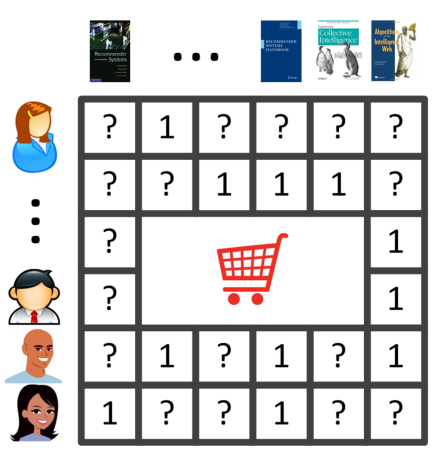
\includegraphics[width=3in]{matrix}
		\caption{user-item 隐式反馈矩阵}
		\label{gra3}
	\end{center}
\end{figure}
在这一节, 我们首先回顾BPR算法,然后讨论它的一些局限性,也就是其收敛缓慢与冷启动问题。通常用户与物品的隐式反馈可以表示为如图\ref{gra3}所示的矩阵, 矩阵的“1”表示用户已经对该物品有过交互行为, 比如购买,点击等, 矩阵的“?”则表示用户还未对该物品有过交互行为。

\subsubsection{Pairwise Preference Assumption}
BPR\cite{rendle2009bpr}是一个应对隐式反馈很流行的推荐框架. 它基于这样一个偏好假设: 如果一个用户$u$已经选择了物品$i$但是没有选择物品$j$,那么在BPR中, 我们认为相对于物品$j$用户$m$更喜欢物品$i$,并定义用户$u$关于物品$i$与$j$的偏好关系为:
\begin{equation}
\label{pairwisepre}
p \left( i \succ_u j \right) := f \left( x_{uij} \right),
\end{equation}
这里$f \left(x\right) = 1/\left(1+exp\left(-x\right)\right)$\footnote{$f \left(x\right)$即为sigmoid函数}, $x_{uij} := s\left(u,i\right) - s\left(u,j\right)$, $s\left(\cdot,\cdot\right)$可以是任何表示用户与物品相关程度的函数。在BPR\cite{rendle2009bpr}中, $s\left(\cdot,\cdot\right)$为用户对物品的预测值, 即$s\left(u,i\right) = \hat{r}_{ui}$, $x_{uij} = \hat{r}_{ui}-\hat{r}_{uj}$.


\subsubsection{预测公式}

在BPR中, 用户$u$对于物品$i$的预测值$\hat{r}_{ui}$公式为:
\begin{equation}
\hat{r}_{ui} = U_{u\cdot}V_{i\cdot}^T + b_i
\end{equation}


\subsubsection{Likelihood of Pairwise Preference}

伯努利分布(Bernouli distribution)是关于布尔变量 $x \in \{0,1\}$ 的概率分布, 其连续参数 $p \in \left[0,1\right]$的概率.
\begin{equation}
\left( x|p \right) = Ber\left(x|p \right)=p^x\left(1-p \right)^{1-x}
\end{equation}

若记事件 $\left(\hat{r}_{ui} > \hat{r}_{uj}\right)$ 的概率为$p\left(\hat{r}_{ui} > \hat{r}_{uj}\right)$, 布尔变量$\delta\left(\left(u,i\right) \succ \left(u,j\right)\right)$ 服从伯努利分布, 那么用户$u$的likelihood of pairwise preference 在\cite{rendle2009bpr}中被定义为:
\begin{equation}
\label{LPP}
\begin{aligned}
LPP_u  
&= \prod_{i,j \ \in \  \mathcal{I}}p\left(\hat{r}_{ui} > \hat{r}_{uj}\right)^{\delta\left(\left(u,i\right) \succ \left(u,j\right)\right)} \left[1-p\left(\hat{r}_{ui} > \hat{r}_{uj}\right)\right]^{1-\delta\left(\left(u,i\right) \succ \left(u,j\right)\right)}\\
&= \prod_{\left(u,i\right) \succ \left(u,j\right)}p\left(\hat{r}_{ui} > \hat{r}_{uj}\right)\prod_{\left(u,i\right) \preceq \left(u,j\right)}\left[1-p\left(\hat{r}_{ui} > \hat{r}_{uj}\right)\right]
\end{aligned}
\end{equation}

这里的$\left(u,i\right) \succ \left(u,j\right)$ 表示用户 $u$ 相比物品 $i$ 更喜欢物品 $j$.

用 $f \left(\hat{r}_{uij} \right)$ 来近似表示概率
$p\left(\hat{r}_{ui} > \hat{r}_{uj}\right)$ \cite{rendle2009bpr}, 对于公式\ref{LPP}取其对数即$\ln LPP_u$, 那么就有:
\begin{equation}
\label{eq5}
\begin{aligned}
\ln LPP_u
&= \ln \prod_{\left(u,i\right) \succ \left(u,j\right)} f \left(\hat{r}_{uij}\right) + \ln \prod_{\left(u,i\right) \preceq \left(u,j\right)}\left[1- f \left(\hat{r}_{uij}\right)\right]\\
&= \ln \prod_{\left(u,i\right) \succ \left(u,j\right)} f \left(\hat{r}_{uij}\right) + \ln \prod_{\left(u,i\right) \succ \left(u,j\right)}\left[1-\left(1- f \left(\hat{r}_{uij}\right)\right)\right]\\
&= \ln \prod_{\left(u,i\right) \succ \left(u,j\right)} f \left(\hat{r}_{uij}\right) + \ln \prod_{\left(u,i\right) \succ \left(u,j\right)} f \left(\hat{r}_{uij}\right)\\
&= 2\ln \prod_{\left(u,i\right) \succ \left(u,j\right)} f \left(\hat{r}_{uij}\right)\\
&= 2 \sum_{i\in\mathcal{I}_u^{tr}}
\sum_{j \in \mathcal{I}\setminus \mathcal{I}_u^{tr}}\ln f \left(\hat{r}_{uij}\right)
\end{aligned}
\end{equation}
在这里$\hat{r}_{uij} = \hat{r}_{ui} - \hat{r}_{uj}$, $f \left(x\right) = 1/\left(1+exp\left(-x\right)\right)$, .

\subsubsection{目标函数}

基于上面的成对偏好假设,可以从隐式反馈数据集中得到所有的偏好集合$D_S := \{\left(u,i,j\right) | v_i \in I_{u}^+ \wedge v_j \in I \setminus I_{u}^+\}$,$I_m^+$表示被用户$u$选择过的物品集合,三元组$\left(u,i,j\right)$表示用户$u$选择过物品$v_i$但是没有选择过物品$v_j$。我们把$v_i$叫做一个positive item,$v_j$叫做一个negative item。对于给定的集合$D_S$, BPR的目标便是最大化所有user-item pair的似然偏好:

\begin{equation}
\label{eq6}
arg \max_{\substack \Theta } \prod_{\left(u,i,j\right) \in D_S} p\left(i \succ_u j\right),
\end{equation}

公式\eqref{eq6}等价于最小化负的对数似然函数:

\begin{equation}
\label{Lfeedback}
L_{feedback} = - \sum_{\left(u,i,j\right) \in D_S}\ln f \left( x_{uij}\right) + \lambda\|\Theta\|^2,
\end{equation}
这里的$x_{uij} = \hat{r}_{uij}$, $\Theta$表示算法中需要学习的模型参数集合,$\lambda$表示超参数集合。在实际的算法学习中, BPR的学习算法经常采用均匀采样的随机梯度下降(\textbf{S}tochastic \textbf{G}radient \textbf{D}escent)进行迭代学习。

更为具体的,公式\eqref{Lfeedback}也就是最小化下面的目标函数(Objective Function): 
\begin{equation}
\label{eq8}
\min_{\substack\Theta}\sum_{u\in\mathcal{U}} \ \sum_{i\in\mathcal{I}_u}\sum_{j\in\mathcal{I}\setminus\mathcal{I}_u}\Phi_{uij}
\end{equation}
这里的
$\Phi_{uij}
= 
- \ln f \left(\hat{r}_{uij}\right) 
+ \frac{\alpha_u}{2}\|U_{u\cdot}\|^2
+ \frac{\alpha_v}{2}\|V_{i\cdot}\|^2
+ \frac{\alpha_v}{2}\|V_{j\cdot}\|^2
+ \frac{\beta_v}{2}\|b_{i}\|^2
+ \frac{\beta_v}{2}\|b_{j}\|^2$, $\Theta = \{U_{u\cdot},V_{i\cdot},b_i\}
$的将要学习的参数集合。


\subsubsection{随机梯度}
对于一个随机采样而得的三元组$\left(u,i,j\right)$, 对目标函数中的参数求其偏导即可得梯度。

在此之前先做一些准备工作,对于函数$f(x) = 1/\left(1+e^{-x}\right)$的导数:

\begin{equation*}
f^{'}(x) = -\frac{1}{\left(1+e^{-x}\right)^2} e^{-x}\left(-1\right) = \frac{e^{-x}}{\left(1+e^{-x}\right)^2} = \frac{1}{\left(1+e^{x}\right)\left(1+e^{-x}\right)} = {f(x)f(-x)}
\end{equation*}

下面开始对参数$U_{u\cdot}$求其偏导:
\begin{equation}
\begin{aligned}
\bigtriangledown U_{u\cdot} 
= \frac{\partial \Phi_{uij}}{\partial U_{u\cdot}}
&=-\frac{\partial \ln f\left(\hat{r}_{uij}\right)}{\partial f\left(\hat{r}_{uij}\right)} 
\frac{\partial f\left(\hat{r}_{uij}\right) }{\partial \hat{r}_{uij}} 
\frac{\partial \hat{r}_{uij}}{\partial U_{u\cdot}}
\ + \  \alpha_uU_{u\cdot}\\
&= -\frac{1}{f\left(\hat{r}_{uij}\right)} 
\frac{\partial f\left(\hat{r}_{uij}\right) }{\partial \hat{r}_{uij}} 
\frac{\partial \hat{r}_{uij}}{\partial U_{u\cdot}}
\ + \  \alpha_uU_{u\cdot}\\
&= -\frac{1}{f\left(\hat{r}_{uij}\right)} 
{f\left(\hat{r}_{uij}\right) f\left(-\hat{r}_{uij}\right)}
\frac{\partial f\left(\hat{r}_{ui} - \hat{r}_{uj}\right) }{\partial U_{u\cdot}} 
\ + \ \alpha_uU_{u\cdot}\\
&= -{f\left(-\hat{r}_{uij}\right)} \frac{\partial f\left[\left(U_{u\cdot}V_{i\cdot}^T+b_i\right) - \left(U_{u\cdot}V_{j\cdot}^T+b_j\right)\right] }{\partial U_{u\cdot}} 
\ + \ \alpha_uU_{u\cdot}\\
&= -{f\left(-\hat{r}_{uij}\right)} \left(V_{i\cdot} - V_{j\cdot}\right)  
\ + \  \alpha_uU_{u\cdot}\\
\end{aligned}
\end{equation}

同样其他参数随机梯度如下:
%\begin{equation}
\begin{align} %align环境不要有空行
\bigtriangledown V_{i\cdot} &= \frac{\partial \Phi_{uij}}{\partial V_{i\cdot}}=-f\left(-\hat{r}_{uij}\right)U_{u\cdot} + \alpha_vV_{i\cdot}\\
\bigtriangledown V_{j\cdot} &= \frac{\partial \Phi_{uij}}{\partial V_{j\cdot}}=-f\left(-\hat{r}_{uij}\right)\left(-U_{u\cdot}\right) + \alpha_vV_{j\cdot}\\
\bigtriangledown b_i        &= \frac{\partial \Phi_{uij}}{\partial b_i} =-f\left(-\hat{r}_{uij}\right)+\beta_vb_i\\
\bigtriangledown b_j        &= \frac{\partial \Phi_{uij}}{\partial b_j} =-f\left(-\hat{r}_{uij}\right)\left(-1\right)+\beta_vb_j
\end{align}
%\end{equation}

\subsubsection{迭代更新}
对于三元组  $\left(u,i,j\right)$ 在采用SGD的BPR算法中的更新公式如下:
%align环境的每行公式默认会进行编号,aligned环境不会
\begin{align}
	\label{eq10}
U_{u\cdot} &= U_{u\cdot} - \gamma\bigtriangledown U_{u\cdot}\\
V_{i\cdot} &= V_{i\cdot} - \gamma\bigtriangledown V_{i\cdot}\\
V_{j\cdot} &= V_{i\cdot} - \gamma\bigtriangledown V_{j\cdot}\\
b_{i\cdot} &= b_i - \gamma\bigtriangledown b_{i}\\
b_{j\cdot} &= b_j - \gamma\bigtriangledown b_{j}
\end{align}

这里的 $\gamma$ 为学习率(learning rate).

\subsubsection{BPR算法}
如算法\ref{al1}即为采用SGD求解的BPR算法。
\IncMargin{1em}
\begin{algorithm}[ht]
	\SetAlgoNoLine %不要算法中的竖线
	\BlankLine
	
	initialize the model parameter $\Theta$\;
	\For {$t_1 = 1,\cdots,T$}{
		\For {$t_2 = 1,\cdots, |\mathcal{P}|$}{
			Randomly pick up a pair $\left(u,v_i\right) \in \mathcal{P}$\;
			Randomly pick up an item $v_j$ from $\mathcal{I} \setminus \mathcal{I}_{u}^+$\;
			Calculate the gradients via Eq.(9-13)\;
			Update the model parameters via Eq.(14-18)\;
		}	
	}
	\caption{The SGD algorithm for BPR}
	\label{al1}%label 放置的位置有讲究, 放后面
\end{algorithm}
\DecMargin{1em}

\subsubsection{收敛缓慢的原因}
由于上面的均匀采样方式会产生很多对于参数学习贡献微弱的train pairs,因此常常会导致收敛缓慢。确切的讲,对于一个给定的训练采样$\left(u,i,j\right) \in D_S$, 由公式\ref{Lfeedback}对随机梯度下降的任意一参数$\theta \in \Theta$求其偏导:

\begin{equation}
\label{eq19}
\frac {\partial L_{feedback}} {\partial\theta} 
= -f\left(-x_{uij}\right)\frac{\partial\left(x_{uij}\right)}{\partial\theta}
= \left(f\left(x_{uij}\right)-1\right) \frac{\partial\left(x_{uij}\right)}{\partial\theta}
\end{equation}

根据公式\eqref{eq19},如果$f \left(x_{uij}\right) \rightarrow +1$,随机梯度将接近于0,则训练采样$\left(u,i,j\right)$对于优化目标的贡献将会变得很小。
\begin{figure}[htbp]
	\begin{center}
		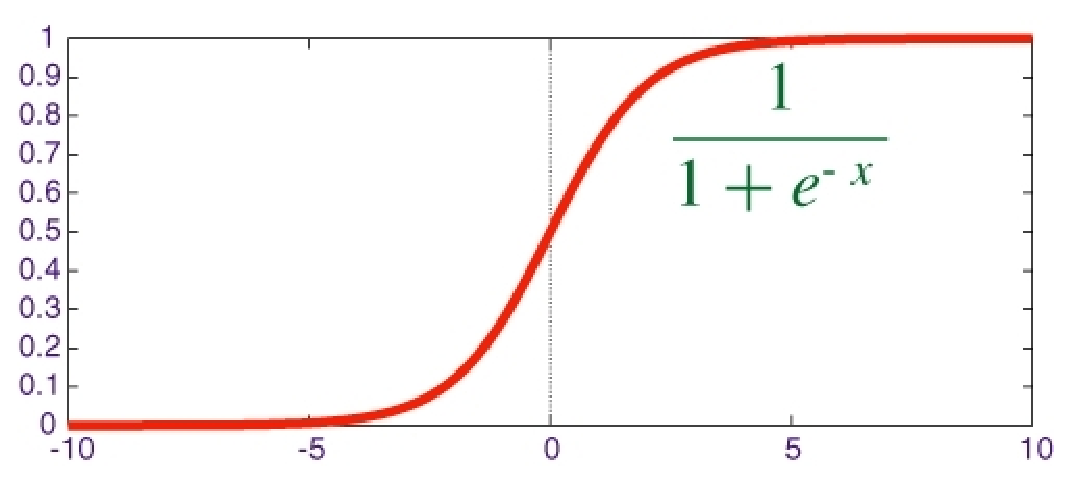
\includegraphics[width=4in]{sigmoid}
		\caption{sigmoid函数$f \left(x\right) $图像}
		\label{gra-sigmoid}
	\end{center}
\end{figure}

联系公式\eqref{eq19}与公式\eqref{pairwisepre},由图\ref{gra-sigmoid} sigmoid函数图像可得, 当$f \left(x_{uij}\right) \rightarrow +1$时, 也就是$x_{uij} = \hat{r}_{ui} - \hat{r}_{uj}$越来越大, 即用户对于物品$v_i$与$v_j$的预测差值越来越大. 因此为了加速学习, 针对一个已有的user-item pair中的物品 $v_i$,要采样的物品$v_j$应当是$v_i$相比有竞争力的物品, 更进一步说也就是由该用户对于$v_i$与$v_j$的偏好得分应该是相近的,否则这个采样对于SGD便是低效的采样。

从经验上来讲,每个用户只会浏览一小部分的物品并对这些浏览过的物品提供一些交互反馈。如果均匀采样器均等地从整个物品集合中采样negative  item.对于一个user-item  pair,大部分均匀采样的物品并不具有可比性或者很难被相关的用户浏览。举个例子,iPhone与牙刷或iPhone与一个冷门的手机品牌可能会经常被均匀采样器采得。而由于这些低效的training pair对于SGD几乎作用很小,整个训练过程便会收敛地极其缓慢。

除此以外,与经典的分解技术相似,如果一个用户或物品缺乏足够的反馈,其对应的隐式表达往往不能够被很好的学习到。在现实世界数据集中,用户行为与物品流行度的分布往往呈现长尾状。这就导致了大部分的用户和物品仅仅有很小部分的反馈数据。此外,在真实的推荐系统中,新的个体可能在任何时间被加入到推荐系统中。因此,BPR框架也很容易受制于冷启动问题。

\subsection{Latent Dirichlet Allocation}
Latent Dirichlet allocation(LDA),隐含狄利克雷分布,是一种主题模型(topic model),它可以将文档集中每篇文档的主题按照概率分布的形式给出。同时它是一种无监督学习算法,在训练时不需要手工标注的训练集,需要的仅仅是文档集以及指定主题的数量即可。此外LDA的另一个优点则是,对于每一个主题均可找出一些词语来描述它。

LDA首先由于2003年提出\cite{blei2003latent},目前在文本挖掘领域包括文本主题识别、文本分类以及文本相似度计算方面都有应用。


\subsubsection{数学模型}
LDA是一种典型的词袋(Bag-of-words)模型,即它认为一篇文档(document)是由一组词(word)构成的一个集合,词与词之间没有顺序以及先后的关系。一篇文档可以包含多个主题(topic),文档中每一个词都由其中的一个主题生成。

\begin{figure}[htbp]
	% caption放上面就会显示在图的上方,出现在下面就是出现在图的下方
	% label的位置也有讲究
	\begin{center}
		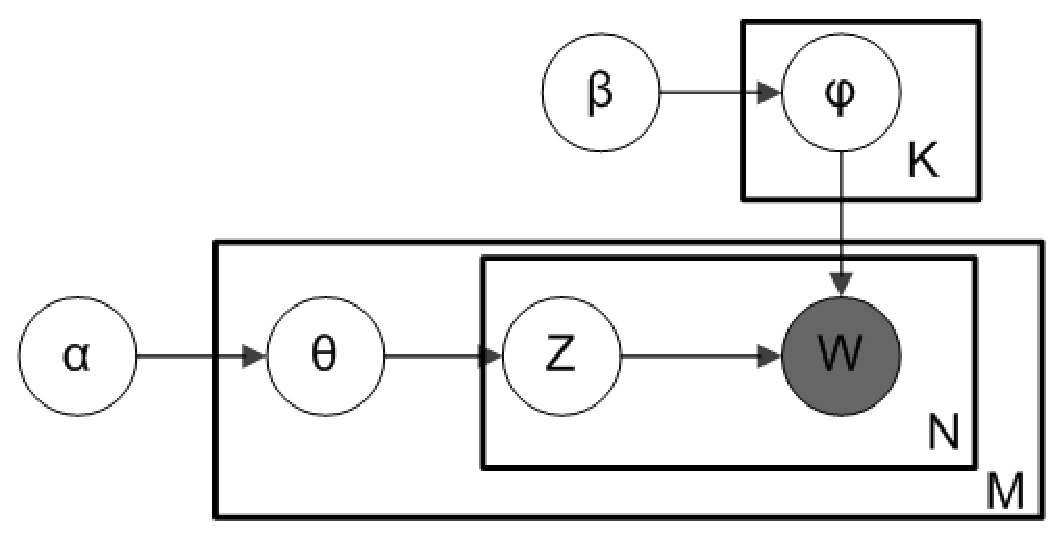
\includegraphics[width=4in]{LDA}
		\caption{LDA 贝叶斯网络结构}
		\label{gra4}
	\end{center}
\end{figure}

另外,正如Beta分布是二项式分布的共轭先验概率分布,狄利克雷分布作为多项式分布的共轭先验概率分布。因此正如图\ref{gra4}, LDA贝叶斯网络结构中所描述的,在LDA模型中一篇文档生成的方式如下:
\begin{itemize}
	\item 从狄利克雷分布$\alpha$ 中取样生成文档$i$的主题分布$\theta_i$
	\item 从主题的多项式分布$\theta_i$中取样生成文档$i$第$j$个词的主题$z_{i, j}$
	\item 从狄利克雷分布$\beta $中取样生成主题$z_{i, j}$的词语分布$\phi_{z_{i, j}}$
	\item 从词语的多项式分布$\phi_{z_{i, j}}$中采样最终生成词语$w_{i, j}$
\end{itemize}
因此整个模型中所有可见变量以及隐藏变量的联合分布是
\begin{equation}
p(w_i, z_i, \theta_i, \Phi | \alpha, \beta) = \prod_{j = 1}^{N} p(\theta_i|\alpha)p(z_{i, j}|\theta_i)p(\Phi|\beta)p(w_{i, j}|\theta_{z_{i, j}})
\end{equation}


最终一篇文档的单词分布的最大似然估计可以通过将上式的$\theta_i$以及$\Phi$进行积分和对$z_i$进行求和得到
\begin{equation}
p(w_i | \alpha, \beta)  = \int_{\theta_i}\int_{\Phi }\sum_{z_i}p(w_i, z_i, \theta_i, \Phi | \alpha, \beta) 
\end{equation}


根据$p(w_i | \alpha, \beta)$ 的最大似然估计,最终可以通过吉布斯采样等方法估计出模型中的参数。


\subsubsection{使用吉布斯采样估计LDA参数}
在LDA最初提出的时候,人们使用EM算法(Expectation-maximization algorithm)进行求解,后来人们普遍开始使用较为简单的Gibbs Sampling,具体过程如下:
\begin{itemize}
	\item 首先对所有文档中的所有词遍历一遍,为其都随机分配一个主题,即$z_{m,n}=k\sim Mult(1/K)$,其中$m$表示第$m$篇文档,$n$表示文档中的第$n$个词,$k$表示主题,$K$表示主题的总数,之后将对应的$n^{\left(k\right)}_m+1$, $n_m+1$, $n^{\left(t\right)}_k+1$, $n_k+1$, 他们分别表示在$m$文档中$k$主题出现的次数,$m$文档中主题数量的和,$k$主题对应的$t$词的次数,$k$主题对应的总词数。
	\item 之后对下述操作进行重复迭代。
	\item 对所有文档中的所有词进行遍历,假如当前文档$m$的词$t$对应主题为$k$,则$n^{\left(k\right)}_m-1$, $n_m-1$, $n^{\left(t\right)}_k-1$, $n_k-1$, 即先拿出当前词,之后根据LDA中topic sample的概率分布sample出新的主题,在对应的$n^{\left(k\right)}_m$, $n_m$, $n^{\left(t\right)}_k$, $n_k$上分别$+1$。
	\begin{equation}
	p(z_i=k|z_{-i},w) \propto k(n^{(t)}_{k,-i}+\beta_t)(n_{m,-i}^{(k)}+\alpha_k)/(\sum_{t=1}^{V}n_{k,-i}^{(t)}+\beta_t)
	\end{equation}
	\item 迭代完成后输出主题--词参数矩阵$\Phi$和文档--主题矩阵$\Theta$
	\begin{align}
	\phi_{k,t}   &=(n_k^{(t)}+\beta_t)/(n_k+\beta_t)  \\
	\theta_{m,k} &=(n_m^{(k)}+\alpha_k)/(n_m+\alpha_k)
	\end{align}
\end{itemize}









\subsection{本章小结}
本章首先介绍了采用SGD求解的Bayesian Personalized Ranking(BPR)推荐算法, 并且对可能导致其收敛缓慢的均匀采样策略做了讨论。然后简要介绍了LDA模型。
	\section{适应性采样策略}
在这一章中,我们结合了内容信息与隐式反馈提出了一个非均匀的物品采样器(a non-uniform item sampler)。在本章中所提出的适应性采样策略(adaptive sampling strategy)自动地模拟了真实的数据分布并且具有适应性地挑选更有针对性的train pairs.


\subsection{适应性采样策略概览}
在现实世界的场景中,用户常常会浏览同一个目录下的多个物品,然后做出他们的选择。那么很显然,我们应该采样具有针对性的物品,比方说针对iPhone,相对于毛巾或者某低档品牌的手机, 采样高档Samsung或者LG显然更具有可比性与合理性。

因此,在适应性采样策略中,我们倾向于采样那些对于用户已选择过的物品更具有可比性同时有很大机会被相关用户浏览的物品。更确切的说,对于一个user-item pair$\left(u_m,v_i\right)$,我们通过以下的步骤采样一个更加合理的负样本(negative item)$v_j$:
\begin{enumerate}
	\item 根据用户$u_m$与物品$v_i$的所在目录分布(categorical distribution),首先推断对于事件用户$u_m$选择物品$v_i$会发生在哪个目录下。
	\item 
	对于给定的一个目录,在该目录下我们进一步选择物品$v_j$作为negative item,而该物品同时又具有较高的概率能够被用户$u_m$所浏览。
\end{enumerate}




\subsection{类别分布}
在适应性采样中, 首先需要知道用户与物品的类别分布(categorical distribution). 不过在有些实际的应用场景中,由于缺乏类别信息,推荐系统并无法直接得到用户与物品的类别分布。为了应对这个问题,我们利用了所谓的隐式表达(the latent representation of an entity)来近似指示其类别信息。

首先我们假设一个entity可能属于多个目录 $C = \{c_1,c_2,\cdots,c_k\}$ ,并且它的类别分布服从幂率(power laws)分布\cite{rendle2014improving}. 用$y_i^e \in \mathbb{R}^k$ 表示 entity $e_i$ 的latent vector ,而矩阵 $Y_e = \left[y_1^e,y_2^e,y_3^e,\cdots\right]$ 是从内容信息(content information)与隐式反馈(implicit feedback)学习得到的entities's latent representation. 以推荐系统中的一个经典场景为例:在推荐系统有两种类型的实体(entity),也就是说用户users, 比如消费者, 和物品items, 比如说电影,书籍和歌曲等。明确起见,本论文使用上标$u$与$v$分别表示与用户user和物品item相关的变量。比如,$y^u_m$表示the latent vector of user $u_m$,$Y^u$表示the latent representation matrix of user, $y_i^v$表示the latent vector of item $v_i$.为了联系categorical distribution 与 the latent vector of entity, 我们认为 entity $e_i$属于目录$c\in C$的概率$p\left(c|e_i\right)$为标准化因子的混合(a mixture over standardized factors),并将其定义为:

\begin{equation}
p\left(c|e_i\right)  \propto exp\left( \frac {y_{i,c}^e - \mu_c}{\sigma_c} \right)
\end{equation}

这里的$\mu_c = E\left(y_{*,c}^e\right)$,$\sigma_c = Var\left(y_{*,c}^e\right)$分别表示all entity factors的经验均值与方差(empirical mean and variance over all entity factors)。假设在用户与物品上的类别分布是相互独立的,那么就可以进一步推断user-item pair$\left(u_m,v_i\right)$同属于一个category $c$的联合概率$p\left(c|u_m,v_i\right)$:

\begin{equation}
\label{eq21}
p\left(c|u_m,v_i\right) = p\left(c|u_m\right)p\left(c|v_i\right)
\end{equation}

根据其联合概率,就可以根据时间用户$u_m$选择物品$v_i$采样一个目录$c$。




\subsection{选取negative item $v_j$}
对于给定一个目录$c$,下一步的目标便是在该目录下选取一个negative item $v_j$,而$v_j$同时将有很大概率会被用户$u_m$所浏览. 

\subsubsection{物品浏览概率}
一个简单点的做法,我们可以将entity $e_i$在目录$c$下的排序得分(ranking score)视作为$p\left(c|e_i\right)$,再进一步从根据它们的排序得分直接选择物品。但实际上,浏览概率(browsing probabilities)与排序得分(ranking scores)并不等同,显然两者之间存在差距。在实际场景中,对于出现在排序列表(ranking lists)中的物品,那些排在靠前位置的物品相对于靠后位置的物品, 往往有着极大的概率被用户所浏览。比如在整个列表中排名前三位的物品的极有可能都会被用户所浏览,而他们排序得分不同的影响在这种情况下将微乎其微。为了应对这个问题,对于给定目录下的物品采样我们分为两步进行:
\begin{enumerate}
	\item 首先,我们先根据经验分布(empirical distribution)从候选物品(candidates)中采样一个排序的位置$r$;
	\item 然后,在该目录下对物品进行排序,返回在位置$r$处的物品作为我们采样的negative item。
\end{enumerate} 

典型地,经验分布大致服从analytical law, 比如Geometric\cite{wang2009pskip}或Zipf\cite{adamic2002zipf} distribution。在这里,我们应用Geometric distribution到从目录$c$的排序列表中选取位置$r(j)$处的物品$v_j$:

\begin{equation}
p\left(v_j|c\right) \propto exp\left(-r\left(j\right)/\lambda\right),\lambda \in \mathbb{R}^+
\end{equation}

这里的$r\left(j\right)$表示物品$v_j$的排序位置,$\lambda$是用来调整概率密度的超参数(hyper-parameter)。




\subsubsection{如何对物品列表进行排序}
在获得negative item的排序位置后,接下来的任务便是如何在这个位置安排对应的物品。\cite{rendle2014improving}中有一个简单的方法:将物品的 latent factors 当作其 ranking scores, 然后根据它们的排序得分(ranking scores)对物品进行排序. 但是由于物品的latent factors在每轮迭代都会被更新,这种方法不得不在每轮迭代每个目录下对物品进行重新排序。这会导致一个很高的计算复杂度,因为每轮迭代需要花费$\mathit{O}\left(kt\log t\right)$的运行时间来进行重新排序,这里的$t$指物品数。为此在\cite{rendle2014improving}中同样提出一个妥协性的做法:每迭代$t \log t$轮再进行重新排序。不过这种妥协会很容易导致局部收敛(local convergence)。此外, 每隔$t\log t$轮进行更新, 实际上在很多未更新的时候的采样相当于从一个随机的物品子集中随机采样, 此时的采样反而会产生副作用。更进一步, 由于items' latent vectors 是被随机初始化, 那么排序列表在首次重排序之前其实是相当于一个随机序列。如果这个随机的排序列表未被及时更新, 那么采样器实际上会衰退为从一个物品子集中随机采样的采样器。因此, 需要一个新的采样方法来平衡效率与推荐表现。

\begin{figure}[htbp]
	\begin{center}
		\includegraphics[width=3.5in]{subspace}
		\caption{将不同模态(different modalities)的entity映射到一个共享的隐式空间(a shared latent space). 在这里假设协同信息(collaborative information), 比如评分(rating), 和内容信息(content information), 比如文本(text),分属于不同模态,正如图中的space A, space B.}
		\label{gra5}
	\end{center}
\end{figure}

根据对于子空间的研究\cite{udupa2010improving,rasiwasia2010new},如果我们将一个entity从不同模态的映射到一个共享子空间,那么它在子空间中的表达应当是具有关联性的,比如互补(complementary)或是相似(similar)。如果我们独立地将一个item从content space和collaborative space映射到a shared latent space,那么我们就能够得到一个item在共享隐式空间的两个latent representations.如图\ref{gra3}所示. 为了避免采样器衰退为从一个物品子集中随机采样一个物品, 我们通过物品的协同信息(collaborative filtering)来初始化排序列表(ranking lists)。具体来说, 我们首先通过特征学习(feature learning)的方法从协同信息中学习物品的一个近似的隐式表达(latent representation), 比如, 用于图像的Conventional Neural Networks(CNN), 用于文本的Latent Dirichlet Allocation(LDA)。那么, 我们将latent factors视作为在目录分布下的物品排序得分, 然后在每个目录下对物品进行排序. 最终, 我们就根据这些排序后的结果对物品排序列表进行初始化。

此外, 为了避免局部收敛的问题, 同时平衡效率, 我们\textbf{只对于那些热门目录下的物品进行重排序}。根据公式\eqref{eq21}, 首先对于一个user-item pair选定一个目录, 然后进一步计算在每个目录下出现了多少所观测的user-item pairs.定义变量$\rho \in \mathbb{R}^k$来表示目录的热度(popularity of categories)。在每次迭代中, 我们根据目录的热度采样出一个热门目录(popular category) $c$:
\begin{equation}
p\left(c|p\right) \propto exp\left(\frac{\rho_c - \mu }{\sigma}\right)
\end{equation}
这里的$\mu$ 和$\sigma$分别表示$\rho$的经验均值与方差(empirical mean and variance). 然后, 我们将物品的current latent factors视为物品的new ranking scores, 并衡量在目录$c$下的new score vector, 根据a similarity function $sim\left(\cdot,\cdot\right)$与旧的score vector相比是否有较大变化.如果ranking score vector的变化超过了阈值 $\delta$, 就用物品的latent represenration matrix 的第$c$列$y_{*,c}^v$来更新在目录$c$下的ranking scores, 并且对该目录下的物品进行重新排序.

\subsection{适应性采样算法}


总言之,在本论文中所研究的适应性采样策略如算法$\ref{al2}$所示, 对于一个user-item pair$\left(u_m,v_i\right)$, 采样一个negative item $v_j$, 而$v_j$与$v_i$相比, 不仅具有可比性,而且具有较高的几率为用户所浏览。在算法$\ref{al2}$中, $index\left(c,r\right)$返回在排序列表$l_c \in L$中位置在$r$处的物品。$x_c \in X$是在目录$c$下的ranking score vector, 而$x_c$正是由从协同信息学习而来approximate latent representation所初始化。值得注意的是, 在整个学习过程中,本论文的适应性采样策略仅需要在一些热门目录重排序几次, 这不仅降低了计算复杂度同时避免了局部极值(local extremum)。

\IncMargin{1em}
\begin{algorithm}
	\SetAlgoNoLine %不要算法中的竖线
	
	\SetKwInOut{Input}{\textbf{输入}}\SetKwInOut{Output}{\textbf{输出}}
	
	\Input{
		\\
		The observed user-item pair set $\mathcal{P}$\;\\
		The counters of category popularity $\rho$\;\\
		The latent representation matrixes $Y^u$ and $Y^v$\;\\
		The ranking scores of items $X = \{x_1,x_2,\cdots,x_k\}$\;\\
		The orders of items $L = \{l_1,l_2,\cdot,l_k\}$\;\\}
	\Output{
		\\
		The training triple $\left(u_m,v_i,v_j\right)$\;\\
		The category popularity $\rho$\;\\
		Draw a category from $p\left(c|\rho\right)$\;\\}
	\BlankLine
	 Draw a popular category $c$ from $p\left(c|\rho\right)$\;
	 \If {$sim \left(x_c,y_{*,c}^v\right) > \delta $}{
		 Update $x_c$ by $y_{*,c}^v$\;
		 Reorder items under $c$ and update $l_c$\;
	 }
	 Draw $\left(u_m,v_i\right) \in \mathcal{P}$ uniformly\;
	 Draw a category $c$ from $p\left(c|u_m,v_i\right)$,$\left(1\leq c \leq k\right)$\;
	 $\rho_c ++$\;
	 Draw a rank $r$ from $p\left(r\right) \propto exp\left(-r/\lambda\right),\left(1\leq c \leq k\right)$\;
	  
	 $v_j \leftarrow 
	 \begin{cases}
	 index\left(c,r\right) & if \ sgn\left(y_{m,c}^u\right) = 1\\
	 index\left(c,n-r-1\right) & else
	 \end{cases}$\;
	 
	\caption{Content-aware and Adaptive sampling}
	\label{al2}
\end{algorithm}
\DecMargin{1em}




\subsection{本章小结}
本章主要介绍了适应性采样策略, 该采样策略通过采样一个具有可比性同时又有较大概率被用户浏览的物品作为negative item。该采样策略不仅能够降低计算复杂度同时能够避免局部极值。
	
	
	
	\bibliographystyle{apalike}
	\bibliography{ref/presentation}
		
\end{document}